Энэ хэсэгт Монгол Ай Ди компанийн хөгжүүлж буй MinuPOS системийн зээлийн хэсэгт харьяалагдах банкны Excel хуулгыг боловсруулах модуль болон түүнтэй холбогдох бодлогыг зохиомжийн үлгэр загваруудыг ашиглан шийднэ.
\section{MinuPOS системийн банкны Excel хуулгыг боловсруулах модулийн шинжилгээ}
Тус модуль нь банкнаас ирсэн Excel файлыг автоматаар уншиж, өгөгдлийг шалган, шаард- лагатай тохиолдолд алдааг илрүүлж, мэдээллийг MinuPOS системийн өгөгдлийн санд шууд хадгалах боломжийг бүрдүүлнэ.
\subsection{MinuPOS системийн танилцуулга}
MinuPOS нь бизнес эрхлэгчид болон жижиг дунд аж ахуйн нэгжүүдийн санхүүгийн хэрэг- цээг хангах цогц зээлийн систем бүхий платформ юм. Эдгээр зээлийн үйлчилгээнүүдийг MinuPOS-ийн мобайл аппликейшн болон POS системээс шууд удирдах боломжтой бөгөөд ингэснээр зээлийн хүсэлт гаргах, төлбөрийн түүхээ харах, POS орлоготой уялдуулан зээлийн төлөлтөө автоматжуулах зэрэг үйлдлийг цахимаар хийх боломжтой.
\subsection{Системийн орчин}

MinuPOS системийн системийн сервер талын код нь Жава технологи дээр бичигдсэн ба үндсэн фреймворк нь Spring Boot юм. MinuPOS нь SoftPOS шийдэлтэй; ухаалаг утсаар карт/NFC төлбөр хүлээн авах боломжийг MineSec SoftPOS\footnote{https://minesecsoftpos.com/}-оор хангадаг.
MinuPOS системийн худалдан авагч/борлуулагч талын интерфэйс нь POS терминал, SoftPOS, нэгдсэн QR дээр суурилна. Борлуулагч талын Монгол Ай Ди компанийн хөгжүүлсэн iOS/Android мобайл аппууд нийтэд байршсан.
MinuPOS систем нь PostgreSQL харьцаат өгөгдлийн санг ашигладаг.

\subsection{Динамик загвар}
MinuPOS системийн банкны Excel хуулгыг боловсруулах модулийн ажлын явцын диаграмыг \ref{fig:module_usecase} зурагт үзүүлэв. 

% @startuml
% left to right direction
% skinparam packageStyle rectangle

% actor Хэрэглэгч as U
% actor Админ as A

% rectangle "\tMinuPOS системийн банкны Excel хуулгыг боловсруулах модуль\t" {
%   usecase "Банкны хуулга оруулах" as UC1
%   usecase "Банкны загвар сонгох" as UC2
%   usecase "Багануудыг буулгах" as UC3
%   usecase "Өгөгдлийг баталгаажуулах" as UC4
%   usecase "Гүйлгээнүүдийг хадгалах" as UC5
%   usecase "Гүйлгээнүүд дээр\n асуулга хийх" as UC6
%   usecase "Банкны загваруудыг \n зохион байгуулах" as UC7
  
%   U --> UC1 : <<include>>
%   U --> UC2 : <<include>>
%   U --> UC3 : <<extend>>\n Хэрэв шинэ загвар\n үүссэн бол
%   U --> UC4
%   U --> UC6
%   A --> UC7 : <<extend>>
  
%   UC1 .> UC2 : <<include>>
%   UC2 .> UC3 : <<extend>>
%   UC3 .> UC4 : <<include>>
%   UC4 .> UC5 : <<include>>
% }
% @enduml

\begin{figure}[h]
		\centering
		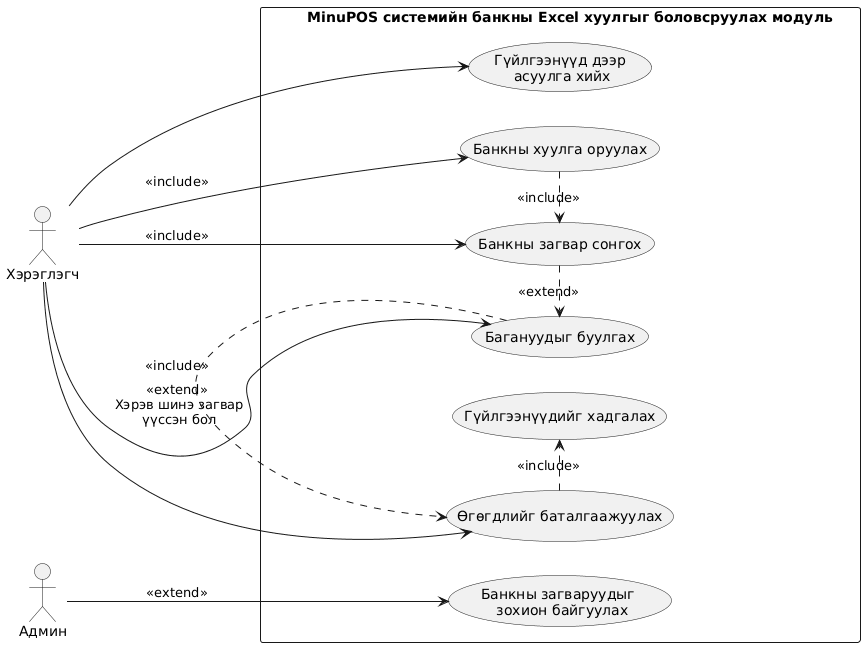
\includegraphics[width=17cm]{images/module_usecase.png}
		\caption{MinuPOS системийн банкны Excel хуулгыг боловсруулах модулийн ажлын явцын диаграм}
		\label{fig:module_usecase}
\end{figure}

Дээрх ажлын явцын диаграмд тусгасан чухал ажлын явцын тайлбаруудыг харгалзах \ref{tab:ucfs01} болон \ref{tab:ucfs02} хүснэгтүүдэд үзүүлэв. Энд ажлын явцын өдөөгч үзэгдэл, тоглогч, угтвар нөхцөл, дараах нөхцөл, үр дүн, тайлбар, өргөтгөл, хувилар болон чанарын шаардлагуудыг тус тус харгалзан үзэв.

%------------------------------------------------------------------------
\begin{longtable}{|L{4cm}|L{\dimexpr\textwidth-4cm-3\tabcolsep-2\arrayrulewidth\relax}|}
\caption{Ажлын явц: Банкны хуулга оруулах (UC-FS-01)}\label{tab:ucfs01}\\ \hline
\textbf{Хэсэг} & \textbf{Агуулга} \\ \hline
\endfirsthead

\multicolumn{2}{c}{\tablename\ \thetable\ -- \textit{үргэлжлэл}} \\ \hline
\textbf{Хэсэг} & \textbf{Агуулга} \\ \hline
\endhead

\hline \multicolumn{2}{r}{\textit{(үргэлжилнэ)}} \\ \hline
\endfoot

\hline
\endlastfoot

Тэмдэглэгээ & UC-FS-01 \\ \hline
Ажлын явцын нэр & Банкны хуулга оруулах \\ \hline
Ангилал & Анхдагч \\ \hline
Тодорхойлолт & Хэрэглэгч нь Монголын 12 банкны аль нэгээс Excel хуулга оруулж, стандарт хэлбэрт шилжүүлэн хадгалах боломжтой. \\ \hline
Өдөөгч үзэгдэл & Хэрэглэгч веб интерфейсээр файл оруулахыг эхлүүлсэн үед \\ \hline
Тоглогч & Банкны хэрэглэгч, Template Mapping үйлчилгээ, Data Validator, PostgreSQL өгөгдлийн сан \\ \hline
Угтвар нөхцөл & 1. Хэрэглэгч нэвтэрсэн байна.\\
               & 2. Банкны загвар байгаа эсвэл үүсгэж болно.\\
               & 3. Файлын хэмжээ $<$ 10\,MB. \\ \hline
Дараах нөхцөл & 1. Гүйлгээний мэдээлэл өгөгдлийн санд хадгалагдсан байна.\\
                & 2. Audit log үүссэн байна.\\
                & 3. Хэрэглэгч үр дүнгийн мэдээлэл авсан байна. \\ \hline
Үр дүн & Стандартчлагдсан санхүүгийн мэдээлэл хэрэглэгчийн атрибутаар хадгалагдсан байна. \\ \hline
Тайлбар & 1. Модуль нь Excel файл болон хэрэглэгчийн сонгосон метадатаг хүлээн авна.\\
              & 2. Метадатагаас банкны төрлийг тодорхойлно.\\
              & 3. Баганын тохиргооны загварыг авна.\\
              & 4. Тохиргооны дүрмээр гүйлгээг задлана.\\
              & 5. Өгөгдлийн бүрэн бүтэн байдал шалгагдана.\\
              & 6. Стандарт $\digamma$ хэлбэрт хөрвүүлнэ.\\
              & 7. Өгөгдлийн санд хадгална.\\ \hline
Өргөтгөл & 3a. Загвар байхгүй тохиолдолд: \\ 
                      & \quad 3a1. Модуль нь баганын тохиргоог асууна. \\ 
                      & \quad 3a2. Хэрэглэгч талбаруудыг тодорхойлно. \\ 
                      & \quad 3a3. Шинэ загвар үүснэ. \\ 
                      & 5a. Буруу өгөгдөл илэрсэн тохиолдолд: \\ 
                      & \quad 5a1. Алдаатай хэсэг хэсгээр импортлогдож тайлан үүснэ. \\ 
                      & \quad 5a2. Хэрэглэгч засаж дахин оруулна. \\ \hline
Хувилар & Өдөөгч: Танигдаагүй файл формат.\\ 
                    & Өдөөгч: Өгөгдлийн сангийн холболт тасарсан.\\ 
                    & Өдөөгч: Засаж болохгүй буруу өгөгдөл. \\ \hline
Чанарын шаардлага & QR-01 (Өгөгдлийн үнэн зөв байдал: 99.9\%)\\ 
          & QR-12 (GDPR нийцтэй байдал)\\ 
          & QR-07 (10,000 бичлэгийг $<$20 секундэд боловсруулна) \\ \hline

\end{longtable}
%------------------------------------------------------------------------
\begin{longtable}{|L{4cm}|L{\dimexpr\textwidth-4cm-3\tabcolsep-2\arrayrulewidth\relax}|}
\caption{Ажлын явц: Банкны загвар үүсгэх (UC-FS-02)}\label{tab:ucfs02}\\ \hline
\textbf{Хэсэг} & \textbf{Агуулга} \\ \hline
\endfirsthead

\multicolumn{2}{c}{\tablename\ \thetable\ -- \textit{үргэлжлэл}} \\ \hline
\textbf{Хэсэг} & \textbf{Агуулга} \\ \hline
\endhead

\hline \multicolumn{2}{r}{\textit{үргэлжнэ}} \\ \hline
\endfoot

\hline
\endlastfoot

Тэмдэглэгээ & UC-FS-02 \\ \hline
Ажлын явцын нэр & Банкны загвар үүсгэх \\ \hline
Ангилал & Анхдагч \\ \hline
Тодорхойлолт & Админ нь шинэ банкны хуулгын форматын баганануудын буулгалтыг тодорхойлж, загвар үүсгэнэ. \\ \hline
Өдөөгч үзэгдэл & Шинэ банк нэмэгдсэн эсвэл форматыг өөрчилсөн тохиолдолд \\ \hline
Тоглогч & Админ \\ \hline
Угтвар нөхцөл & 1. Админ нэвтэрсэн байна.\\
               & 2. Жишиг хуулга бэлэн байна.\\
               & 3. Стандарт талбарууд тодорхойлогдсон байна. \\ \hline
Дараах нөхцөл & 1. Шинэ загвар хувилбар хадгалагдсан байна.\\
                & 2. Хэрэглэгчдэд мэдэгдсэн байна.\\
                & 3. Өөрчлөлтийн лог бүртгэгдсэн байна. \\ \hline
Үр дүн & Банкны хуулгад ашиглах дахин ашиглах боломжтой буулгалт бүхий загвар үүссэн байна. \\ \hline
Тайлбар & 1. Админ жишиг хуулгыг оруулна.\\
              & 2. Модуль нь баганын толгойн мөрийг гаргаж авна.\\
              & 3. Админ багануудыг стандарт талбаруудад буулгана.\\
              & 4. Модуль нь буулгалтын бүрэн бүтэн байдлыг шалгана.\\
              & 5. Загвар хадгалагдана.\\ \hline
Өргөтгөл & 4a. Буулгалт гүйцээгүй тохиолдолд: \\
                      & \quad 4a1. Модуль нь дутагдсан талбаруудыг онцолж харуулна. \\
                      & \quad 4a2. Админ нэмэлт буулгалт оруулна. \\[4pt]
                      & 5a. Өмнөх загвартой зөрчилдөөн гарвал: \\
                      & \quad 5a1. Хувилбаруудын харьцуулалтыг харуулна. \\
                      & \quad 5a2. Админ давхарлах эсэхийг баталгаажуулна. \\ \hline
Хувилбар & Өдөөгч: Буруу буулгалт тохиргоо.\\
                    & Өдөөгч: Хадгалах квота хэтэрсэн. \\ \hline
Чанарын шаардлага & QR-09 (загвар үүсгэх хугацаа $<$ 5 минут)\\
          & QR-14 (Хувилбар зөрчилөөс урьдчилан сэргийлэх)\\
          & QR-03 (Zero-downtime шинэчлэлтүүд) \\ \hline

\end{longtable}


\newpage
\subsection{Функциональ  шаардлага}
Доор MinuPOS системийн банкны Excel хуулгыг боловсруулах модулийн функциональ шаардлагуудыг жагсаав.
\begin{table}[h]
\caption{MinuPOS системийн банкны Excel хуулгыг боловсруулах модулийн функциональ шаардлага}
\begin{tabular}{|p{3cm}|p{13cm}|}
\hline
Шаардлагын нэр & \text{Шаардлагын тайлбар} \\ \hline
ФШ10 & Модуль нь банкны Excel хуулгаас гүйлгээний мэдээллийг (огноо, дүн, тайлбар) уншиж авна. \\ \hline
ФШ11 & Модуль нь өгөгдсөн банкны Excel хуулгаас уншиж авсан мэдээллийг  $\digamma$ стандарт бүтэцтэй объектод хувиргана. $\digamma$ стандарт бүтцийн дэлгэрэнгүйг "Өгөгдлийн бүтэц ба загвар" хэсгээс харна уу. \\ \hline
ФШ12 & Модуль нь өгөгдсөн банкны Excel хуулгын мэдээллийг өгөгдлийн санд хадгалдаг байна. \\ \hline
ФШ13 & Хэрэв сонгосон банкны төрөлд тохирохгүй Excel загвар хуулагдвал, модуль хэрэглэгчид алдааны мэдээлэл харуулна. \\ \hline
ФШ14 & Хэрэв Excel файлд буруу дүн эсвэл огноо байвал, модуль тухайн мэдээллийг алдаатай гэж тэмдэглэж харуулна. \\ \hline
ФШ20 & Модуль нь хэрэглэгчээс банкны төрлийг оролтоор авдаг байна. \\ \hline
ФШ21 & Модуль нь хэрэглэгчид банкны Excel хуулгын загварыг оролтоор оруулах боломжийг олгодог байна. \\ \hline
ФШ30 & Модуль нь хэрэглэгчээс банкны Excel хуулгыг оролтоор авдаг байна. \\ \hline
\end{tabular}
\end{table}

\newpage
\subsection{Функциональ бус шаардлага}
Доор MinuPOS системийн банкны Excel хуулгыг боловсруулах модулийн функциональ бус шаардлагуудыг жагсаав.
\begin{table}[h]
\caption{MinuPOS системийн банкны Excel хуулгыг боловсруулах модулийн функциональ бус шаардлага}
\begin{tabular}{|p{3cm}|p{13cm}|}
\hline
Шаардлагын нэр & \text{Шаардлагын тайлбар} \\ \hline
ФШБ10 & 1000 хүртэлх мөр бүхий Excel хуулгыг 5 секундын дотор боловсруулж, өгөгдлийн санд амжилттай хадгалдаг байна. \\ \hline
ФБШ11 & Модуль нь ачааллын үеэр ч тогтвортой ажиллаж, хариу өгөх хугацаа 2 секундээс хэтрэхгүй байна. \\ \hline
ФБШ12 & Банкны Excel хуулганд агуулагдах нийт гүйлгээний тоо 10000-д хүрэх үед ч системийн ажиллагаа алдагдахгүй байна. \\ \hline
ФБШ20 & Хэрэглэгчийн Excel хуулга оруулах үйлдэл нь ойлгомжтой, 3-аас илүүгүй алхмаар хийгддэг байна. \\ \hline
ФБШ30 & Алдаа гарсан тохиолдолд өгөгдлийн алдагдлаас урьдчилан сэргийлж, 30 секундын дотор ажлыг үргэлжлүүлдэг байна. \\ \hline
ФБШ40 & Модуль нь шинэ банкны төрөл эсвэл загварыг нэмэхэд хялбар, үүнийг хийхэд одоо байгаа кодонд их хэмжээний өөрчлөлт хийх шаардлагагүй байна. \\ \hline
ФБШ41 & Код нь цэгцтэй, тайлбар бичигдсэн, өөр хөгжүүлэгч тухайн кодыг ойлгоход хялбар байна. \\ \hline
\end{tabular}
\end{table}
\newpage
\subsection{Өгөгдлийн бүтэц ба загвар}
MinuPOS системийн банкны Excel хуулгыг боловсруулах модуль нь $\digamma$ стандарт бүтэцтэй өгөгдлийн загварыг ашиглана. $\digamma$ стандарт бүтэц нь дараах төрөл бүхий талбарыг агуулна:
\subsubsection{Банкны хуулгын өгөгдлийн баганууд}
\begin{table}[h]
\centering
\caption{MinuPOS системийн $\digamma$ стандарт бүтцийн толгой баганууд}
\begin{tabular}{|p{5cm}|p{5cm}|}
\hline
\textbf{Баганы нэр} & \textbf{Өгөгдлийн төрөл} \\ \hline
STATEMENT\_ID & VARCHAR2(20) \\ \hline
REQUEST\_ID & VARCHAR2(20) \\ \hline
BANK\_CODE & VARCHAR2(20) \\ \hline
START\_DATE & DATE \\ \hline
END\_DATE & DATE \\ \hline
TXN\_COUNT & NUMBER \\ \hline
INCOME & NUMBER \\ \hline
OUTCOME & NUMBER \\ \hline
FILE\_ID & VARCHAR2(100) \\ \hline
ACCOUNT\_NO & VARCHAR2(20) \\ \hline
CREATED\_DATE & DATE \\ \hline
STATEMENT\_DATE & DATE \\ \hline
MAIN\_FLAG & VARCHAR2(2) \\ \hline
ACCOUNT\_NAME & VARCHAR2(200) \\ \hline
\end{tabular}
\end{table}
\newpage
\subsubsection{Банкны хуулгын гүйлгээний дэлгэрэнгүй баганууд}
\begin{table}[h]
\centering
\caption{MinuPOS системийн $\digamma$ стандарт бүтцийн дэлгэрэнгүй баганууд}
\begin{tabular}{|p{5cm}|p{5cm}|}
\hline
\textbf{Баганы нэр} & \textbf{Өгөгдлийн төрөл} \\ \hline
DETAIL\_ID & VARCHAR2(20) \\ \hline
STATEMENT\_ID & VARCHAR2(20) \\ \hline
TXN\_DATE & DATE \\ \hline
PRE\_BALANCE & NUMBER \\ \hline
POST\_BALANCE & NUMBER \\ \hline
TXN\_AMOUNT & NUMBER \\ \hline
TXN\_TYPE & VARCHAR2(20) \\ \hline
TXN\_DESC & VARCHAR2(1000) \\ \hline
CO\_ACCOUNT & VARCHAR2(200) \\ \hline
USE\_FLAG & VARCHAR2(2) \\ \hline
USE\_FLAG\_USER\_ID & VARCHAR2(20) \\ \hline
USE\_FLAG\_DATE & DATE \\ \hline
STATUS & VARCHAR2(20) \\ \hline
\end{tabular}
\end{table}

\subsection{Модулийн динамик загвар}



\section{Модулийн архитектур, зохиомж}

\section{Модулийн хэрэгжүүлэлт}